%----------------------------------------------------------------------------------------
%	KOPPEN EN BIJLAGE
%----------------------------------------------------------------------------------------
\newpage

\section{Hoofdstuk 3}									%Het titel van het hoofdstuk - plaats deze alleen wanneer deze samenvatting over de eerst sectie gaat.

\subsection{3.2 Optellen en aftrekken - Shakirullah Hamza}							%De titel van de sectie / paragraaf uit het boek en de naam van de samenvatter.
												        %Hanteer bij voorkeur dezelfde sectienummers als in het boek!
\begin{wrapfigure}{r}{0pt}
\attachfile{hoofdstuk.tex}									%Bijvoegen van het oorspronkelijke .tex bestand, pas bestandsnaam waar nodig aan.
\end{wrapfigure}

%----------------------------------------------------------------------------------------
%	SAMENVATTING
%----------------------------------------------------------------------------------------
Alle verwijzingen naar bladzijdes zijn over Editie 5 van het boek

\textbf{Optellen}: 1+0 = 1	1+1= 0 (1 carry)		1+1+1=1 (1 carry)
\textbf{Aftrekken}: Hetzelfde als bij decimalen of je kan optellen via de two’s complements regel. 

Bij het optellen van getallen met verschillende tekens kan er geen overflow ontstaan, omdat de som niet groter kan zijn dan een van de operanden.
Bij aftrekken geldt het tegenovergestelde, er kan geen overflow ontstaan als beide tekens van de getallen hetzelfde zijn.

\textbf{Hoe herken je overflows?}
- Als bij het optellen van 2 positieve getallen het resultaat een negatief getal is en vice versa.
- Als we een negatief getal van een positief getal aftrekken en een negatief resultaat krijgen
- Als we een positef getal van een negatief getal aftrekken en een positef resultaat krijgen

ADD, ADDI, SUB veroorzaken exceptions bij overflow.
ADDU, ADDIU, SUB veroorzaken geen exceptions bij overflow
Exceptions worden gebruikt om overflow te detecteren.

Omdat C overflows negeert, geven de MIPS C compilers altijd een UNSIGHNED versie van de instructies ADDU,ADDIU,SUBU.
Sommige computers hebben saturating, hierbij wordt bij overflow het resultaat veranderd naar de hoogste toelaatbare waarde of de laagste toelaatbare waarde.
							                %Typ hier de samenvatting van een hoofdstuk of sectie / paragraaf.
\subsection{3.3 vermenigvuldigen - Shakirullah Hamza}						
\begin{wrapfigure}{r}{0pt}
\attachfile{hoofdstuk.tex}									
\end{wrapfigure}

%----------------------------------------------------------------------------------------
%	SAMENVATTING
%----------------------------------------------------------------------------------------

Vermenigvuldigen gaat hetzelfde als bij decimalen.
De vermenigvuldigtal en de vermenigvuldiger worden geshift twerijl de vermenigvuldigtal opgeteld wordt bij het product als de verminigvuldiger bit 1 is. 
Algoritme:
\usepackage{graphicx}
\graphicspath{{/afbeeldingen}}
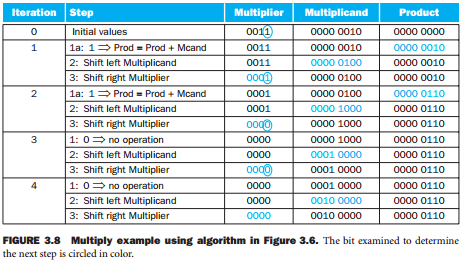
\includegraphics{1} 

blz 187
\newpage

hardware

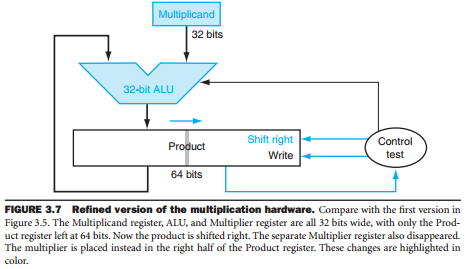
\includegraphics{2}

dit is verfijnd blz 186, eerste versie staat op blz 184

\subsection{3.4 Delen - Shakirullah Hamza}							
												       
\begin{wrapfigure}{r}{0pt}
\attachfile{hoofdstuk.tex}									
\end{wrapfigure}

%----------------------------------------------------------------------------------------
%	SAMENVATTING
%----------------------------------------------------------------------------------------

Hetzelfde algoritme dat bij decimalen wordt gebruikt.

Hardware:

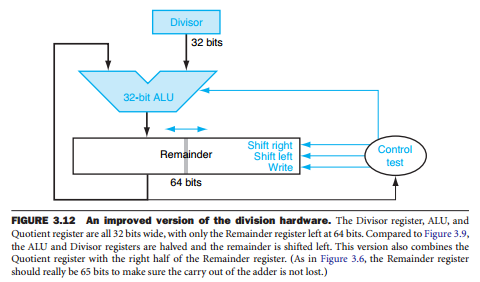
\includegraphics{3}

dit is verfijnd blz 192, eerste versie blz 190

algoritme:

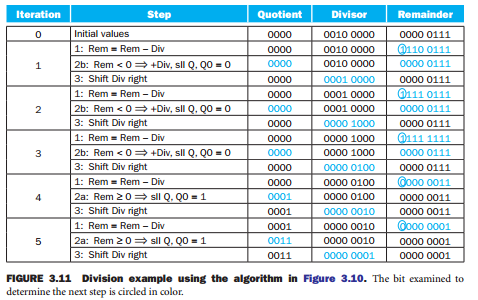
\includegraphics{4}

blz 192

\textbf{Signed delen}:
De divident en de restwaarde moeten dezelfde teken hebben (+/-)

\textbf{Delen in Mips}:

Hi bewaart de restwaarde

Lo bewaart het quotient


\subsection{3.5 Floating Point - Shakirullah Hamza}							%De titel van de sectie / paragraaf uit het boek en de naam van de samenvatter.
												        %Hanteer bij voorkeur dezelfde sectienummers als in het boek!
\begin{wrapfigure}{r}{0pt}
\attachfile{hoofdstuk.tex}									%Bijvoegen van het oorspronkelijke .tex bestand, pas bestandsnaam waar nodig aan.
\end{wrapfigure}

%----------------------------------------------------------------------------------------
%	SAMENVATTING
%----------------------------------------------------------------------------------------

\textbf{Voordelen van genormaliseerde wetenschappelijke notaties}:

- Het maakt verwisselen van data die floating point numbers inhouden makkelijker.

- Het maat floating point arithmetic algorithms simpeler, wetend dat de getallen altijd in deze form zullen zijn

- Het verhoogt de precisie van nummers die in een word bewaard worden, omdat onnodig leidende Nullen vervangen worden.

Een designer moet een compromis vinden tussen de grootte van de fractie en de groote van de exponent. De trade-off is tussen precisie en bereik. Het vergrootten van de fractie vergroot de precies en de grootte van de exponent vergroot het bereik van de nummers die gerepresenteerd worden.

\textbf{Notaties}:

Wetenschappelijke notatie: X.Y * 10^n

Genormaliseerde notatie: X,Y * 10^n (X = GEEN NUL)

Overflow in floatingpoint: exponent is te groot
Underflow in floatingpoint: Negatieve exponent is te groot.

Een manier om overflow/underflow te verminderen is een ander formaat te gebruiken met een groter exponent: Double precision.

\textbf{Double precision} is een floating point getal die gerepresentateerd wordt in twee 32-bit words.

\textbf{Single precision}:	s = 1 bit		exponent = 8 bits	fractie = 23 bits 	bias : 127

\textbf{Double precision}:	s = 1 bit		exponent = 11 bits	fractie = 32 bits		bias : 1023

Hoewel double precision de exponent vergroot, is de grootste voordeel dat precisie vergroot wordt door de hogere fractie.

Vorm floating points numbers in het algemeen:		(-1)^S * F * 2^E

\textbf{Floating point optellen}: 

1.	Exponenten gelijk maken

2.	Optellen (zoals bovenaan)

3.	De som in genormaliseerde notatie zetten.

4.	Afronden


\textbf{Floating point vermenigvuldigen}:

1.	Exponent gelijk maken	(exponenten optellen)

2.	Vermenigvuldigen	(zoals bovenaan)

3.	Normaliseerde notatie

4.	Afronden

5.	Teken hang af van de originele getallen ( teken gelijk aan elkaar = positief, anders negatief)


\subsection{3.9 Pitfalls and Fallacies - Shakirullah Hamza}							
												        
\begin{wrapfigure}{r}{0pt}
\attachfile{hoofdstuk.tex}									
\end{wrapfigure}

\textbf{Fallacy}: Net als dat een left shift instructie een integer vermenigvuldigt met een macht van 2 kan vervangen, is de right shift hetzelfde als een integer delen door een macht van 2.
Dit is waar voor unsigned integers maar een probleem bij signed integers.

\textbf{Pitfall}: Floating-point optelling is niet associatief
Omdat getallen met een groot bereik gerepresenteerd kunnen worden in floating point, worden er problemen veroorzaijkt als je 2 grote getallen met een klein getal optelt.

\textbf{Fallacy}: Parallel execution strategies die werken voor een integer data type werken ook voor floating-point data typen
Verschillende aantal processors geven alleen hetzelfde resultaat bij two’s complent integers omdat integers optellingen associatief zijn. Floating point optellingen zijn niet associatief.

\textbf{Pitfall}: De MIPS instructie ADDIU sign exten zijn 16-bit immediate field
ADDIU is gebruikt om constanten bij signed integers op te tellen als we geen zorgen maken om overflow.

\textbf{Fallacy}: Alleen theoretisch wiskundigen maken zich zorgen over floating point precisie
Andere mensen gebruiken ook floating point precisie.
